\documentclass[12pt,french]{report}
%%%%%%%%%%%%%%%%%%%%%%%%%%%%%%%%%%%%%%%%%%%%%%%%%%%%%%%%%%%%%%%%%%%%%%%%%%%%%%%
\input{preambule_2020}
\portrait
%%%%%%%%%%%%%%%%%%%%%%%%%%%%%%%%%%%%%%%%%%%%%%%%%%%%%%%%%%%%%%%%%%%%%%%%%%%%%%%

\fancyhf{}
\rhead{ \textcolor{orange!90}{\bsc{\large Algorithmes}}}
\lhead{}
\rfoot{TP Algo}
\lfoot{Seconde}
\cfoot{\thepage / \pageref{LastPage}}
\renewcommand \headrulewidth{0pt}
\renewcommand {\footrule}{{\color{orange!70}\rule{\textwidth}{0.9pt}}\\}
\pagestyle{fancy}

%%%%%%%%%%%%%%%%%%%%%%%%%%%%%%%%%%%%%%%%%%%%%%%%%%%%%%%%%%%%%%%%%%%%%%%%%%%%%%%

\newcommand{\casiotriangle}[2]{\raisebox{#1em}{
\begin{tikzpicture}[scale=#2]
\tkzDefPoint(0,0){A}
\tkzDefPoint(1,0){B}
\tkzDefPoint(1,1){C}
\tkzDrawPolygon[fill=black](A,B,C)
\end{tikzpicture}
}
}


\usepackage[linesnumbered,french]{algorithm2e}
%%%%%%%%%%%%%%%%%%%%%%%%%%%%%%%%%%%%%%%%%%%%%%%%%%%%%%%%%%%%%%%%%%%%%%%%%%%%%%%

%%%%%%%%%%%%%%%%%%%%%%%
%% DEBUT DU DOCUMENT %%
%%%%%%%%%%%%%%%%%%%%%%%

\begin{document}

\begin{module}[colback=blue!10]{TP Algo}
\vspace*{1em}
\begin{center}
\textcolor{blue}{\huge \bsc{Différentes présentations d'algo}}
\end{center}
\vspace*{0.2em}
\end{module}

%%%%%%%%%%%%%%%%%%%%%%%%%%%%%%%%%%%%%%%%%%%%%%%%%%%%%%%%%%%%
\begin{spacing}{1.2}
%%%%%%%%%%%%%%%%%%%%%%%%%%%%%%%%%%%%%%%%%%%%%%%%%%%%%%%%%%%%


\begin{center}
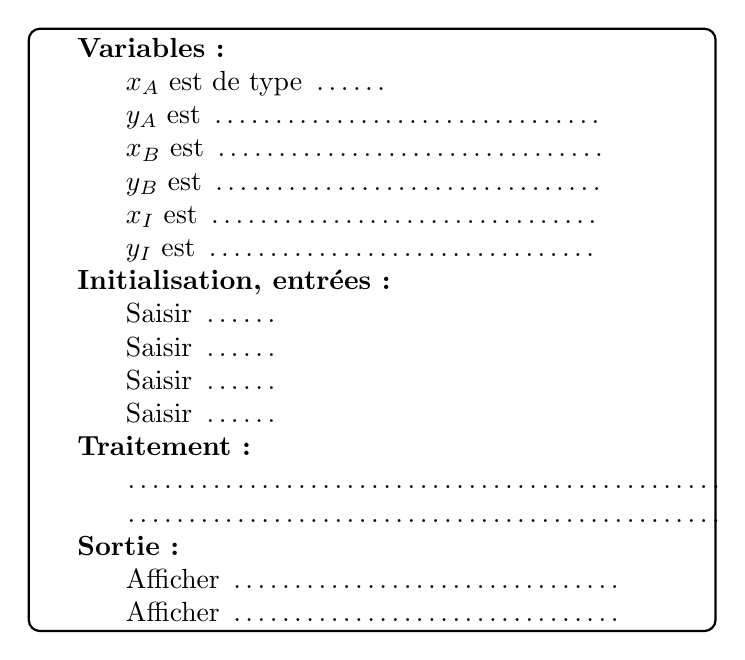
\begin{tikzpicture}
\node[rectangle,draw=black,rounded corners,thick,fill=white]{%
\begin{minipage}{0.7\linewidth}
\hspace*{0.5cm}\textbf{Variables :} \\
      \hspace*{1cm} $x_A$ est de type \makebox[1cm]{\dotfill} \\
      \hspace*{1cm} $y_A$ est \makebox[5cm]{\dotfill} \\
      \hspace*{1cm} $x_B$ est \makebox[5cm]{\dotfill} \\
      \hspace*{1cm} $y_B$ est \makebox[5cm]{\dotfill} \\
      \hspace*{1cm} $x_I$ est \makebox[5cm]{\dotfill} \\
      \hspace*{1cm} $y_I$ est \makebox[5cm]{\dotfill} \\
\hspace*{0.5cm}\textbf{Initialisation, entrées :} \\
      \hspace*{1cm} Saisir \makebox[1cm]{\dotfill} \\
      \hspace*{1cm} Saisir \makebox[1cm]{\dotfill} \\
      \hspace*{1cm} Saisir \makebox[1cm]{\dotfill} \\
      \hspace*{1cm} Saisir \makebox[1cm]{\dotfill} \\
\hspace*{0.5cm}\textbf{Traitement :} \\
      \hspace*{1cm} \makebox[0.9\textwidth]{\dotfill} \\
      \hspace*{1cm} \makebox[0.9\textwidth]{\dotfill} \\
\hspace*{0.5cm}\textbf{Sortie :} \\
      \hspace*{1cm} Afficher \makebox[5cm]{\dotfill} \\
      \hspace*{1cm} Afficher \makebox[5cm]{\dotfill}
\end{minipage}
};\end{tikzpicture}

\end{center}

Voici les algorithmes version \og calculatrice\fg~ pour la question \ding{173} :\\

\textbf{Nouvelle commande !!} \verb=\casiotriangle=\,

\begin{center}
\begin{mybox}[colback=blue!10]{ALGO}
\begin{small}\begin{center}
\begin{mybox}[colback=blue!10]{ALGO}
\textbf{Variables :} \\
      \hspace*{1cm} $x$, $y$  sont des réels\\
\textbf{Initialisation, entrées :} \\
      \hspace*{1cm} $-1\longrightarrow x$\\
      \hspace*{1cm} $x^3-5x\longrightarrow y$ \\
\textbf{Traitement :} \\
      \hspace*{1cm} Tant que $y>3$ Faire\\
      \hspace*{2cm}\makebox[0.2\textwidth]{\dotfill}$\longrightarrow x$ \\
      \hspace*{2cm}\makebox[0.2\textwidth]{\dotfill}$\longrightarrow y$ \\
      \hspace*{1cm} Fin Tant que \\
\textbf{Sortie :} \\
      \hspace*{1cm} Afficher $(x-0,01\pv x)$
\end{mybox}
\end{center}

\begin{multicols}{2}
\textbf{Avec une TI :}\\

:Input "Nombre à dépasser",A\\
:3000 $\rightarrow$ S\\
:0 $\rightarrow$ N\\
:While  U$\leq$A\\
:1,04S+350 $\rightarrow$ S\\
:N+1$\rightarrow$N\\
:End\\
:Disp "On dépassera la somme au bout de :",N,"années"

\columnbreak

\textbf{Avec une Casio :}\\

"Nombre à dépasser"\RetourChariot\\
?$\rightarrow$A\RetourChariot\\
3000 $\rightarrow$ S\RetourChariot\\
0 $\rightarrow$ N\RetourChariot\\
While  S$\leq$A\RetourChariot\\
1,04S+350 $\rightarrow$ S\RetourChariot\\
N+1$\rightarrow$N\RetourChariot\\
WhileEnd\RetourChariot\\
"On dépassera la somme au bout de :" \casiotriangle{0}{0.2}\\
N \casiotriangle{0}{0.2}\\
"années"\RetourChariot

\end{multicols}					
					
\end{small}					
\end{mybox}
\end{center}

\begin{center}
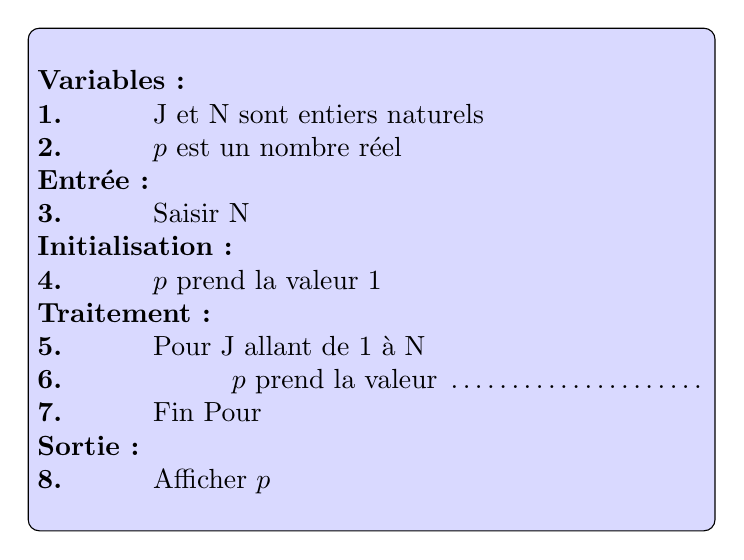
\begin{tikzpicture}
\node[rectangle,draw,rounded corners,fill=blue!15]{
\begin{minipage}{0.7\textwidth}
\vspace{12pt}
\textbf{Variables :}\\
\textbf{1.}\hspace{1cm} J et N sont entiers naturels\\
\textbf{2.}\hspace{1cm} $p$ est un nombre réel\\
\textbf{Entrée :}\\
\textbf{3.}\hspace{1cm} Saisir N\\
\textbf{Initialisation :}\\
\textbf{4.}\hspace{1cm} $p$ prend la valeur 1\\
\textbf{Traitement :}\\
\textbf{5.}\hspace{1cm} Pour J allant de 1 à N\\
\textbf{6.}\hspace{2cm} $p$ prend la valeur \dotfill\\
\textbf{7.}\hspace{1cm} Fin Pour\\
\textbf{Sortie :}\\
\textbf{8.}\hspace{1cm} Afficher $p$\\
\end{minipage}
};
\end{tikzpicture}
\end{center}





\begin{center}
\begin{mybox}[colback=blue!10]{ALGO}
\textbf{Variables :} \\
      \hspace*{1cm} $x$, $y$  sont des réels\\
\textbf{Initialisation, entrées :} \\
      \hspace*{1cm} $-1\longrightarrow x$\\
      \hspace*{1cm} $x^3-5x\longrightarrow y$ \\
\textbf{Traitement :} \\
      \hspace*{1cm} Tant que $y>3$ Faire\\
      \hspace*{2cm}\makebox[0.2\textwidth]{\dotfill}$\longrightarrow x$ \\
      \hspace*{2cm}\makebox[0.2\textwidth]{\dotfill}$\longrightarrow y$ \\
      \hspace*{1cm} Fin Tant que \\
\textbf{Sortie :} \\
      \hspace*{1cm} Afficher $(x-0,01\pv x)$
\end{mybox}
\end{center}


\begin{center}
\begin{mybox}[colback=blue!10]{ALGO}
\begin{lstlisting}[language=Python]
# Calcul de la factorielle
def factorielle(x):
	if x < 2:
		return 1
	else:
		return x * factorielle(x-1)
str(5) + "! = " + str(factorielle(5))
\end{lstlisting}
\end{mybox}
\end{center}

\begin{center}
\begin{mybox}[colback=blue!10]{ALGO}
\begin{verbatim}
# Calcul de la factorielle
def factorielle(x):
    if x<2:
        return 1
    else:
        return x*factorielle(x-1)
str(5)+"! = "+str(factorielle(5))
\end{verbatim}
\end{mybox}
\end{center}


\begin{center}
\begin{minipage}{0.55\linewidth}
\begin{mybox}[colback=blue!10]{ALGO}


\end{mybox}
\end{minipage}
\end{center}


\textbf{Avec algorithm2e}

%\begin{minipage}{.45\linewidth}
%%\begingroup \removelatexerror% Nullify \@latex@error %Pour mettre des algo en mode twocolumns %ou bien enlever [H]
%\RestyleAlgo{boxed} %boxed, boxruled, ruled and algoruled.
%\NoCaptionOfAlgo %supprime le titre en dessous de l'algo
%\begin{algorithm}[H] %version * : met l'algo à cheval sur 2 colonnes en mode twocolumns %options [Hhtbp]
%\DontPrintSemicolon %n'affiche pas les ; en fin de ligne
%%\SetAlgoNoLine %Enlève des filets verticaux et met les blocs de "fin"
%%\SetAlgoVlined %Conserve les filets verticaux avec crochet retour et enlève les blocs de "fin" % A EVITER
%\SetAlgoLined  %Conserve les filets verticaux et met les blocs de "fin"
%
%$n$ et $i$ sont des entiers naturels \;
%$u$ et $S$ sont des nombres réels \;
%Entrer $n$ \;
%$u \leftarrow 0$ ; $S \leftarrow 0$ ; $n \leftarrow 1$ \;
%\Tq{$i<n$}{
%$u \leftarrow 2u+1-i$ \;
%$S \leftarrow S+u$ \;
%$i \leftarrow i+1$ \;
%}
%\Pour{i \KwDe {\rm 1} \KwA N}{
%$y$ reçoit $a×i+b$ \;
%Afficher \og f(\fg $i$ \og)=\fg $y$ \;
%}
%Afficher $(u;S)$
%%\caption{\bfseries Algorithme 1} %Titre de l'algo ; supprimé par
%\NoCaptionOfAlgo
%\end{algorithm}
%%\endgroup
%\end{minipage} 



\normalem %%%% disable auto underline
\DontPrintSemicolon %n'affiche pas les ; en fin de ligne
%\SetAlgoNoLine %Enlève des filets verticaux et met les blocs de "fin"
\SetAlgoVlined %Conserve les filets verticaux avec crochet retour et enlève les blocs de "fin" % A EVITER
%\SetAlgoLined  %Conserve les filets verticaux et met les blocs de "fin"
%\RestyleAlgo{ruled} %boxed, boxruled, ruled and algoruled.

\hspace*{2em}\textbf{Algorithme MaxCompatible(S)}

\hspace*{3em}\begin{algorithm}[H]
$S' \leftarrow 0$\;
Trier les activités de S par durée croissante\;
\Pour{$i$ de 1 à $\abs{S}$}{
\Si{l'activité $i$ est compatible avec les activités de $S'$}{
Ajouter l'activité $i$ à $S'$
}
}
\end{algorithm}
\ULforem %%%% enable auto underline



\begin{center}
\begin{minipage}{0.45\linewidth}
\begin{mybox}[colback=blue!10]{Algorithme de dichotomie}
\normalem %%%% disable auto underline
\DontPrintSemicolon %n'affiche pas les ; en fin de ligne
%\SetAlgoNoLine %Enlève des filets verticaux et met les blocs de "fin"
\SetAlgoVlined %Conserve les filets verticaux avec crochet retour et enlève les blocs de "fin" % A EVITER
%\SetAlgoLined  %Conserve les filets verticaux et met les blocs de "fin"
%\RestyleAlgo{ruled} %boxed, boxruled, ruled and algoruled.

\hspace*{0.5em}\begin{algorithm}[H]
Entrer $a$, $b$, $p$\;
\Tq{$b-a>p$}{
$\dfrac{a+b}{2}\rightarrow c$

\Si{$f(c)\times f(a)>0$}{
$c\rightarrow a$}
\Sinon{$c\rightarrow b$}
}
\end{algorithm}
\ULforem %%%% enable auto underline
\end{mybox}
\end{minipage}
\end{center}

%%%%%%%%%%%%%%%%%%%%%%%%%%%%%%%%%%%%%%%%%%%%%%%%%%%%%%%%%%%%
\end{spacing}
%%%%%%%%%%%%%%%%%%%%%%%%%%%%%%%%%%%%%%%%%%%%%%%%%%%%%%%%%%%%
%%%%%%%%%%%%%%%%%%%%%
%% FIN DU DOCUMENT %%
%%%%%%%%%%%%%%%%%%%%%
\end{document}